\section{Model Exercise 2-1a (02): Fluid driven percolation in salt}
\label{sec:mex02}
%------------------------------------------------------------------------------
\Authors{Amir Shoarian Sattari, Mathias Nest, Keita Yoshioka et al.}
%------------------------------------------------------------------------------
Model Exercise 2 (ME 2) investigates the fluid driven percolation (hydraulic fracking) in salt and clay stone samples under anisotropic confining stresses. The pressurized oil is injected through the pre-drilled cavity until the sudden pressure drop or increase in flow rate is observed. The main goal of this test is to determine the stress dependent fracking path and the required fracking pressure which should be higher than the minimum principle stress applied to the system. For the simulation of the fluid driven percolation, the continuum and discreet methods are considered.
%------------------------------------------------------------------------------
\subsection{Experimental set-up}
%------------------------------------------------------------------------------
The experimental tests on rock salt samples have been conducted at the IfG Leipzig \cite{Kamlot2009}. The cubic samples with a side length dimension of 100 $mm$ are prepared and placed in the true tri-axial apparatus (Fig. \ref{fig:Amir_ME2_Saltstone_Setup}). The cubic samples are prepared with a drilled cavity with a length of 40 $mm$ and a diameter of 16 $mm$. The pressurized fluid is injected through a tubing from the top and the fracking and change of flow rate is tracked. The applied two anisotropic stress configurations and the fracking paths are shown in  Fig. \ref{fig:Amir_ME2_stress_state_a} and \ref{fig:Amir_ME2_stress_state_b}. Fig. \ref{fig:Amir_ME2_Pressure_Time_a} and \ref{fig:Amir_ME2_Pressure_Time_b} depict the change of pressure inside of the borehole with time under the constant flow rate sequels.

\begin{figure}[!ht]
\centering
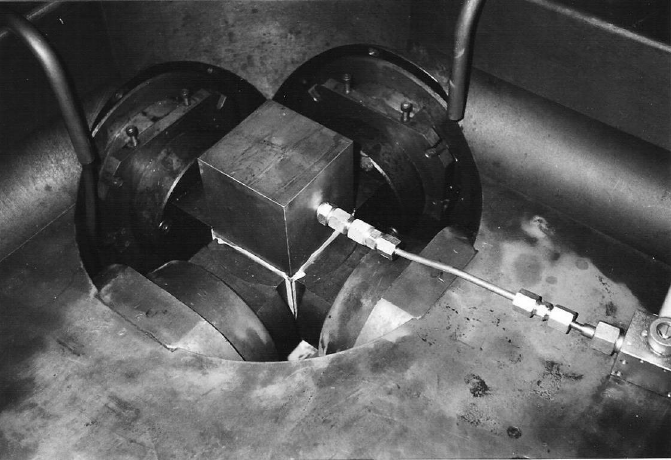
\includegraphics[width=0.5\textwidth]{figures/Amir_ME2_Saltstone_Setup.png}
\caption{ME2 setup configuration of saltstone placed inside the true tri-axial apparatus \cite{Kamlot2009}}
\label{fig:Amir_ME2_Saltstone_Setup}
\end{figure}

\begin{figure}[!ht]
\begin{subfigure}[c]{0.48\textwidth}
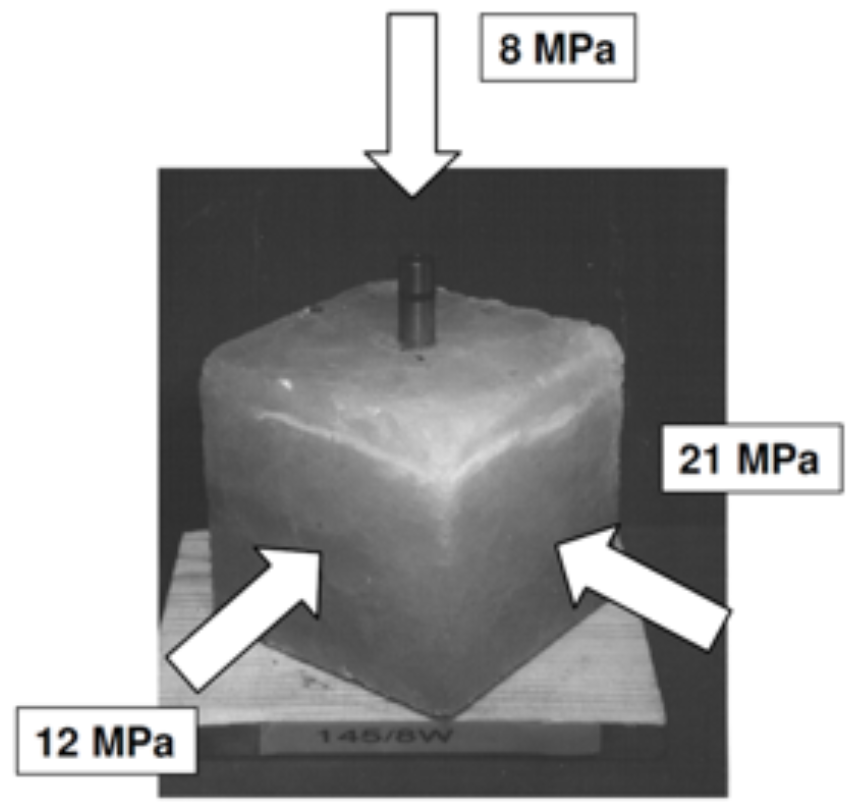
\includegraphics[width=1\textwidth]{figures/Amir_ME2_stress_state_1.png}
\subcaption{}
\label{fig:Amir_ME2_stress_state_a}
\end{subfigure}
\hfill
\begin{subfigure}[c]{0.48\textwidth}
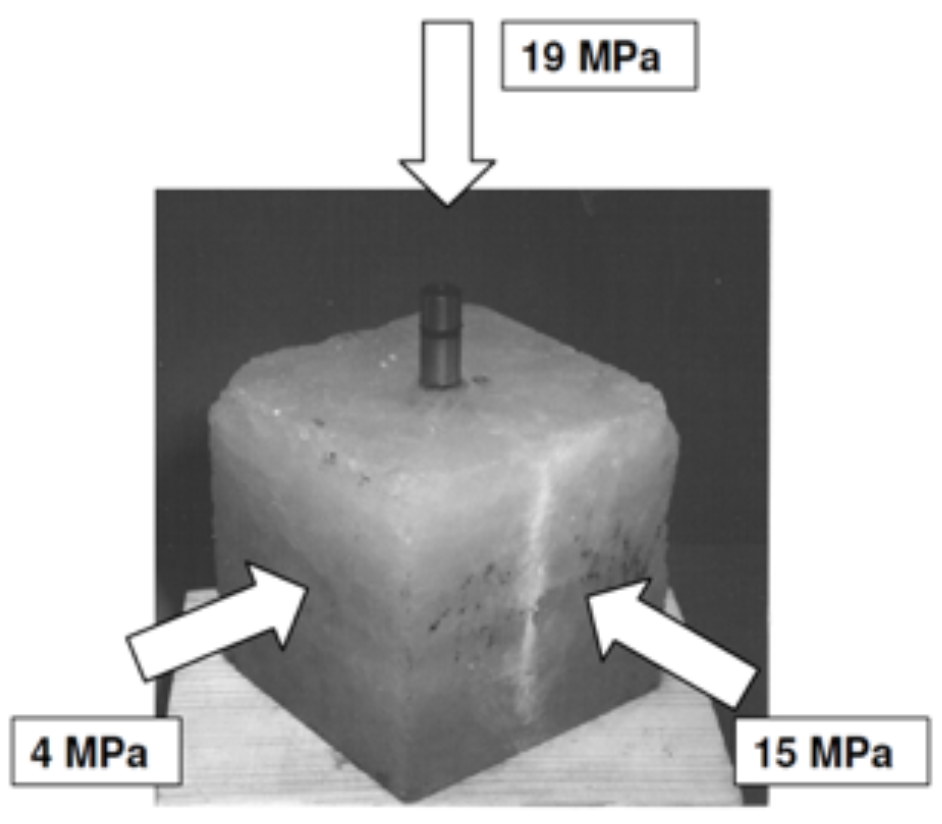
\includegraphics[width=1\textwidth]{figures/Amir_ME2_stress_state_2.png}
\subcaption{}
\label{fig:Amir_ME2_stress_state_b}
\end{subfigure}
\caption{The confining (a) $1^{st}$ stress, and (b) $2^{nd}$ stress configuration setup in saltstone \cite{Kamlot2009}}
\end{figure}

\begin{figure}[!ht]
\begin{subfigure}[c]{0.48\textwidth}
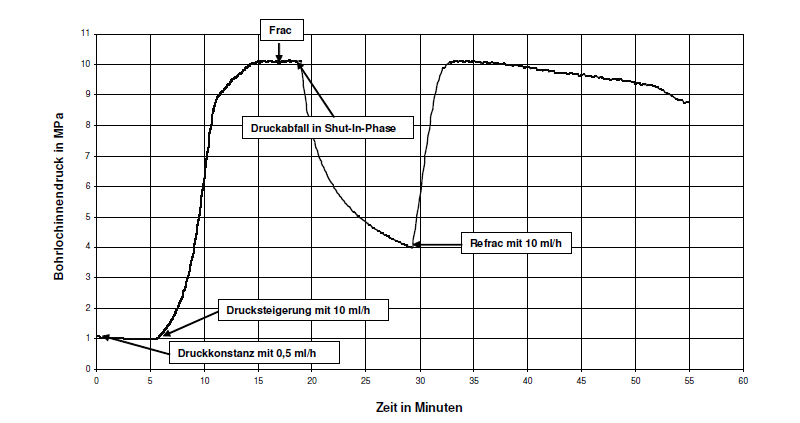
\includegraphics[width=1\textwidth]{figures/Amir_ME2_Pressure_Time_1.png}
\subcaption{}
\label{fig:Amir_ME2_Pressure_Time_a}
\end{subfigure}
\hfill
\begin{subfigure}[c]{0.48\textwidth}
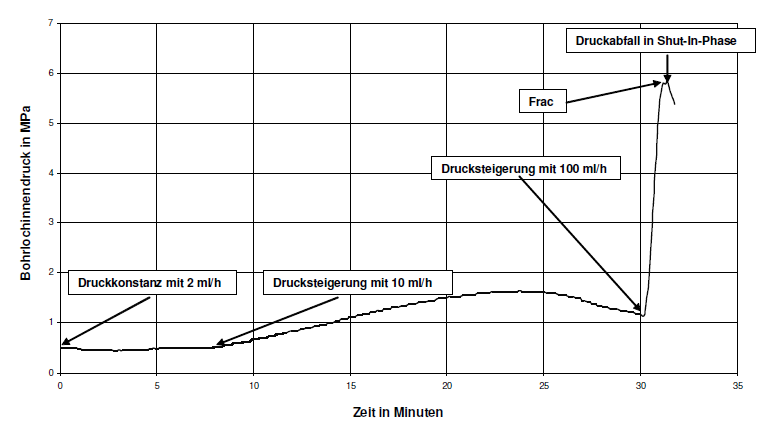
\includegraphics[width=1\textwidth]{figures/Amir_ME2_Pressure_Time_2.png}
\subcaption{}
\label{fig:Amir_ME2_Pressure_Time_b}
\end{subfigure}
\caption{The borehole pressure evolution under constant flow rate sequels for (a) $1^{st}$ stress, and (b) $2^{nd}$ stress configurations \cite{Kamlot2009}}
\end{figure}
%------------------------------------------------------------------------------
\subsection{Model approaches}
%------------------------------------------------------------------------------
Different numerical methods (DEM, LEM, PFM) are implemented to investigate the applicability of each model to simulate the fracking path, fracking pressure and flow rate changes in the saltstone samples. Below, the description of each model and the discussion of the results are provided. The stress dependent fracking path due to anisotropic stress configurations are captured by both continuum and discrete models. 
%------------------------------------------------------------------------------
\subsubsection*{Discrete-Element-Model (DEM)}
Figure \ref{fig:ME2_DEM_model_setup} shows the elements and interfaces/grain boundaries used for the DEM simulation of this modeling exercise. For both of the stress states, the identical elements and interfaces were used. Simulation results from the first stress configuration are shown in Fig. \ref{fig:ME2_DEM_stress1_result}.

\begin{figure}[!ht]
\centering
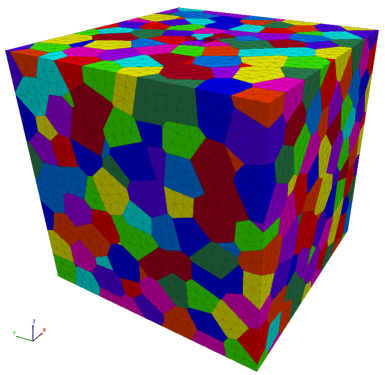
\includegraphics[width=0.45\textwidth]{figures/ME2_DEM_model.pdf}
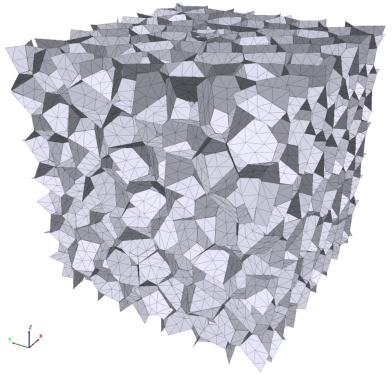
\includegraphics[width=0.45\textwidth]{figures/ME2_DEM_grain.pdf}
\caption{ME2 DEM model set-up.}
\label{fig:ME2_DEM_model_setup}
\end{figure}

\begin{figure}[!ht]
\centering
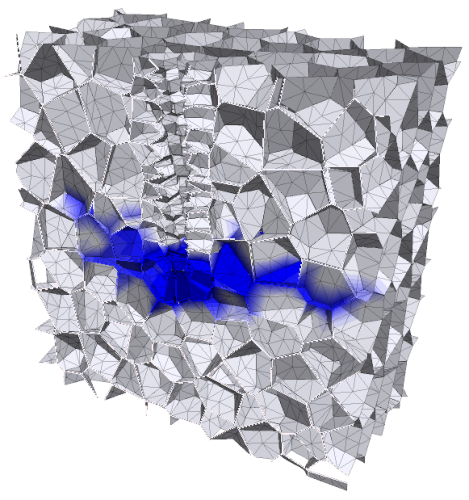
\includegraphics[width=0.45\textwidth]{figures/ME2_DEM_stress1_vertical.pdf}
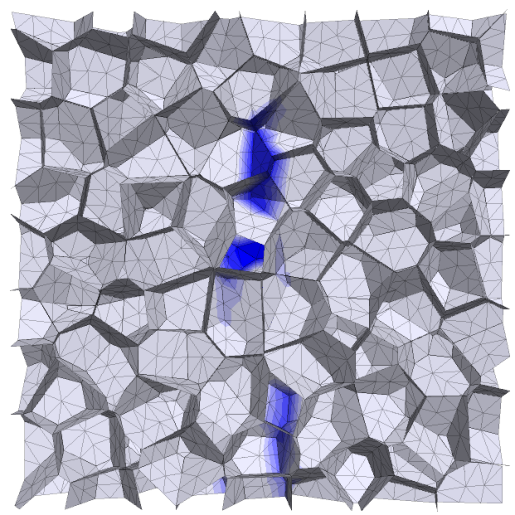
\includegraphics[width=0.45\textwidth]{figures/ME2_DEM_stress2_side.pdf}
\caption{ME2 DEM model results for the stress configuration 2.}
\label{fig:ME2_DEM_stress1_result}
\end{figure}

\begin{figure}[!ht]
\centering
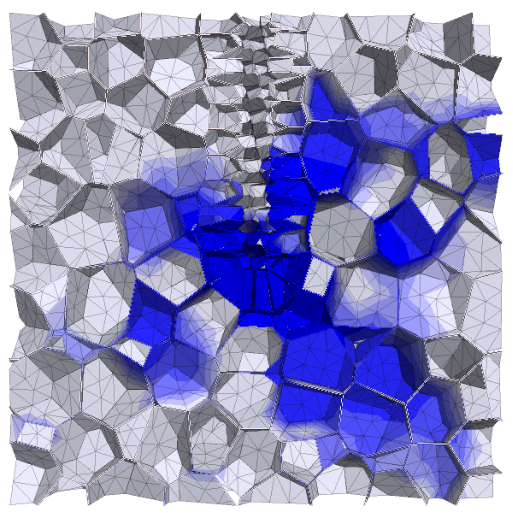
\includegraphics[width=0.45\textwidth]{figures/ME2_DEM_stress2_vertical.pdf}
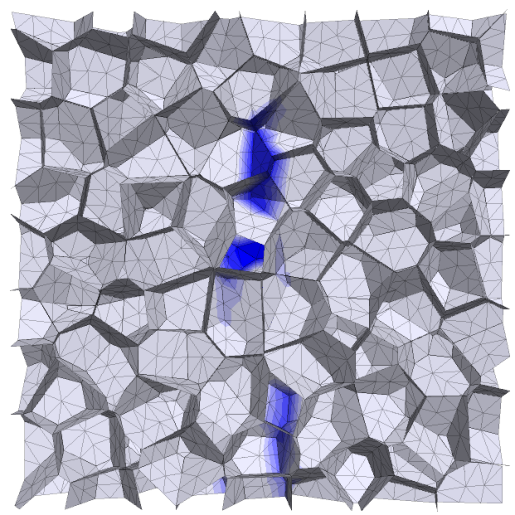
\includegraphics[width=0.45\textwidth]{figures/ME2_DEM_stress2_side.pdf}
\caption{ME2 DEM model results for the stress configuration 2.}
\label{fig:ME2_DEM_stress2_result}
\end{figure}

\subsubsection*{Lattice-Element-Model (LEM)}

The dual lattice model, described in the section \ref{Section:HMLattice}, is implemented to simulate the fluid driven percolation in the saltstone samples. The applied hydraulic pressures are transformed into the mechanical model using the weak coupling scheme and subsequently the elements failure and change of hydraulic aperture are determined and transformed back to the hydro model. The considered mass conservation law results in the prediction of flow rate and change of reservoirs pressure as well as the flow and fracking paths, which are then compared to the experimental data. The total number of mechanical and conduct lattice elements are approximately 6000 and 45000, respectively (\ref{fig:Amir_ME2_LEM_a_model}).  The experimental setup shown in Fig. \ref{fig:Amir_ME2_stress_state_a} is simulated using  the dual LEM and the developed fracture surfaces are shown in Fig. \ref{fig:Amir_ME2_LEM_a_model_Fracture}. Similarly, the fracture surfaces under the second stress configuration (Fig. \ref{fig:Amir_ME2_stress_state_b}) are illustrated in Fig. \ref{fig:Amir_ME2_LEM_b_model_Fracture}. In these simulations the Young's modulus is assumed to be 30 $GPa$. While comparing the experimental and the numerical results, the frack propagation along the horizontal axis (visible on the surface frack path) for the $1^{st}$ stress configuration (Fig. \ref{fig:Amir_ME2_LEM_a_model_Fracture}) is observed. In Fig. \ref{fig:Amir_ME2_LEM_b_model_Fracture}, the fracking path propagation in the vertical direction (visible on the surface frack path) similar to the experimental result (Fig. \ref{fig:Amir_ME2_stress_state_b}) is observed.  

\begin{figure}[!ht]
\centering
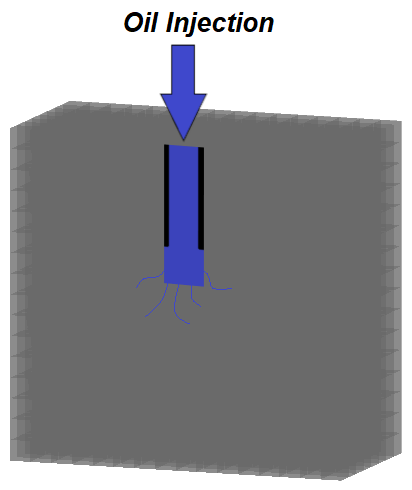
\includegraphics[width=4cm,height=5cm]{figures/Amir_ME2_LEM_a_model.png}
\caption{The boundary condition in the lattice model, cross-section view}
\label{fig:Amir_ME2_LEM_a_model}
\end{figure}

\begin{figure}[!ht]
\begin{subfigure}[c]{0.48\textwidth}
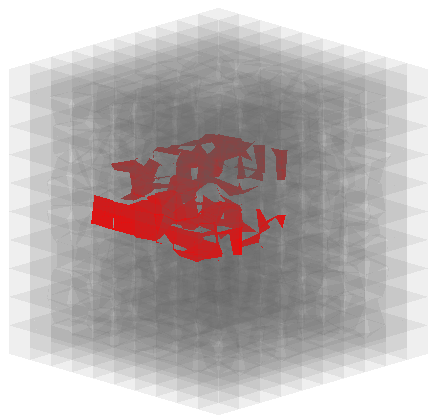
\includegraphics[width=5cm,height=5cm]{figures/Amir_ME2_LEM_a_model_Fracture.png}
\subcaption{}
\label{fig:Amir_ME2_LEM_a_model_Fracture}
\end{subfigure}
\hfill
\begin{subfigure}[c]{0.48\textwidth}
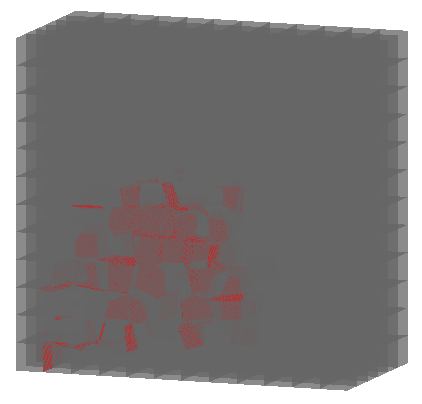
\includegraphics[width=5cm,height=5cm]{figures/Amir_ME2_LEM_b_model_Fracture.png}
\subcaption{}
\label{fig:Amir_ME2_LEM_b_model_Fracture}
\end{subfigure}
\caption{The simulation of the fluid driven percolation and developed frack surfaces (red) for the (a) $1^{st}$, and (b) $2^{nd}$ stress configurations}
\end{figure}

%------------------------------------------------------------------------------
\subsubsection*{Finite-Element-Model: Variational-Phase-Field (VPF)}
%------------------------------------------------------------------------------
A computational domain for the variational phase-field model is depicted in Fig~\ref{fig:VPF_init}.
Relying on the symmetry of the domain, 1/4 of the domain was simulated. 
The whole domain was discretized with first-order tetrahedral elements.
The total element count is 27,917,126 with 5,432,325 nodes.
Two scenarios of boundary loading as in Figs~\ref{fig:Amir_ME2_stress_state_a} and~\ref{fig:Amir_ME2_stress_state_b} were simulated  .

\begin{figure}[!ht]
\centering
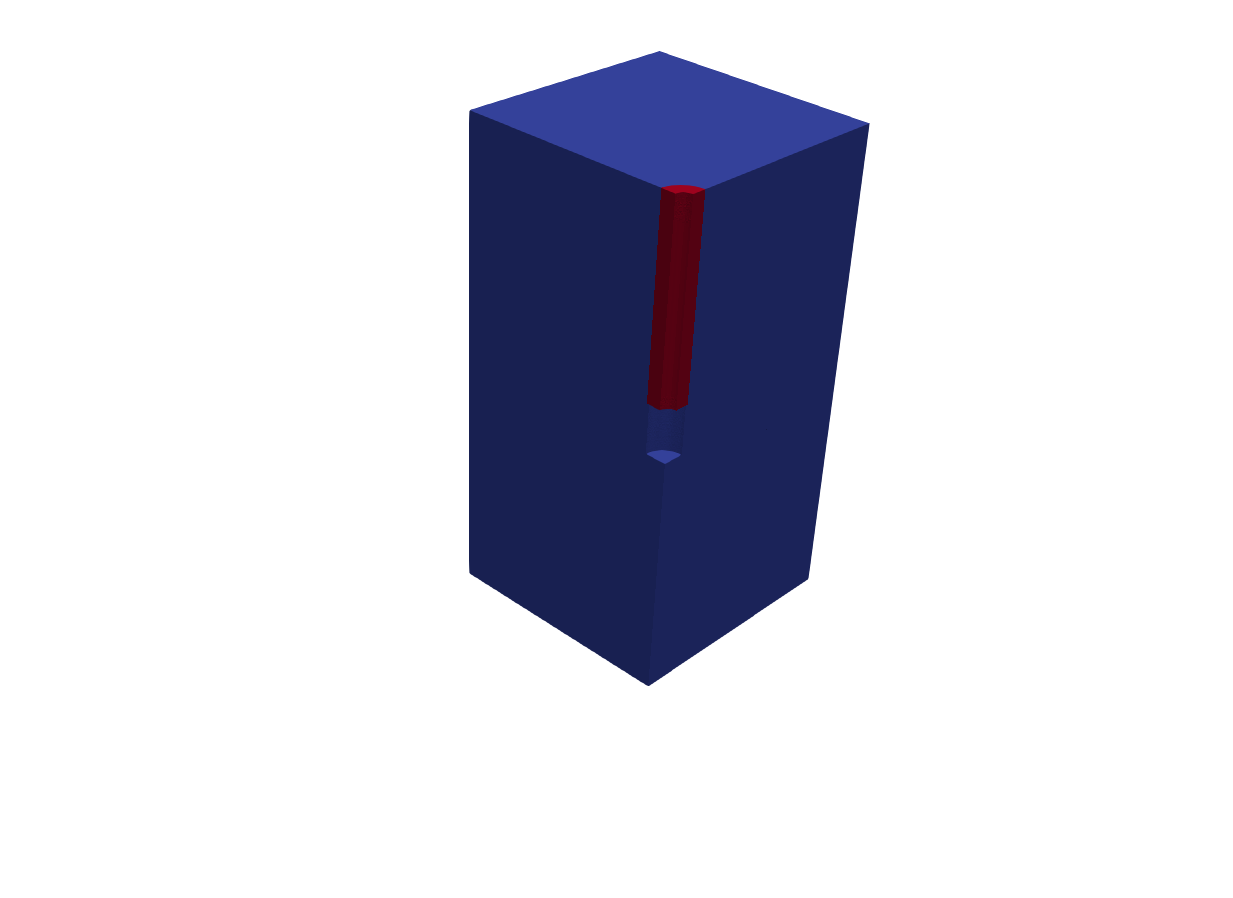
\includegraphics[width=1.0\textwidth]{figures/VPF_init.png}
\caption{A computational domain for the variational phase-field model.}
\label{fig:VPF_init}
\end{figure}

\begin{figure}[!ht]
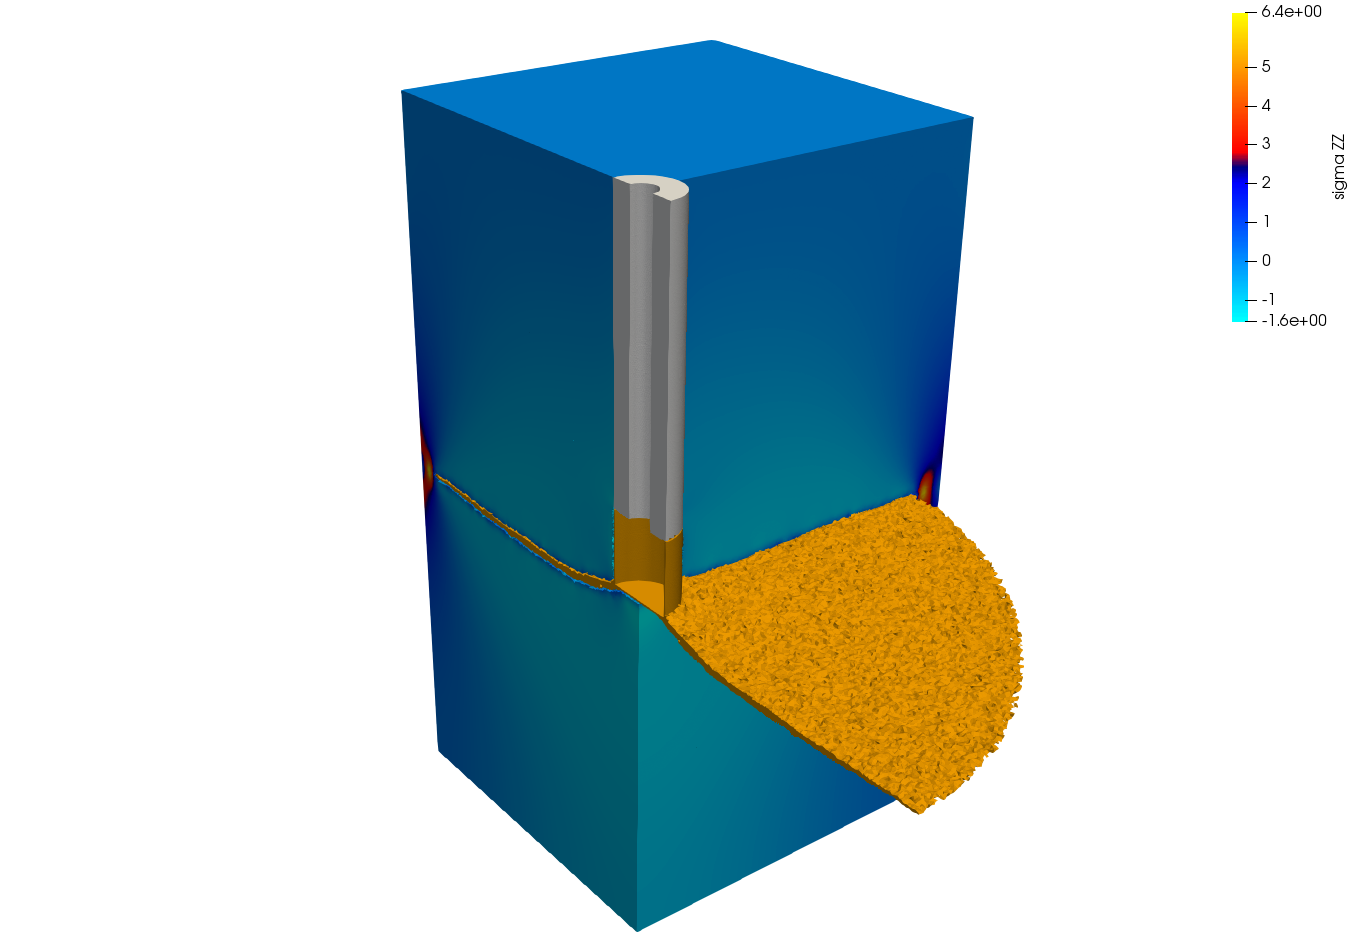
\includegraphics[width=1\textwidth]{figures/VPF_ME2_case1.png}
\caption{The simulation of fluid driven percolation for case1. Created fracture and the vertical stress are shown.}
\label{fig:Keita_ME2_VPF_case1}
\end{figure}

\begin{figure}[!ht]
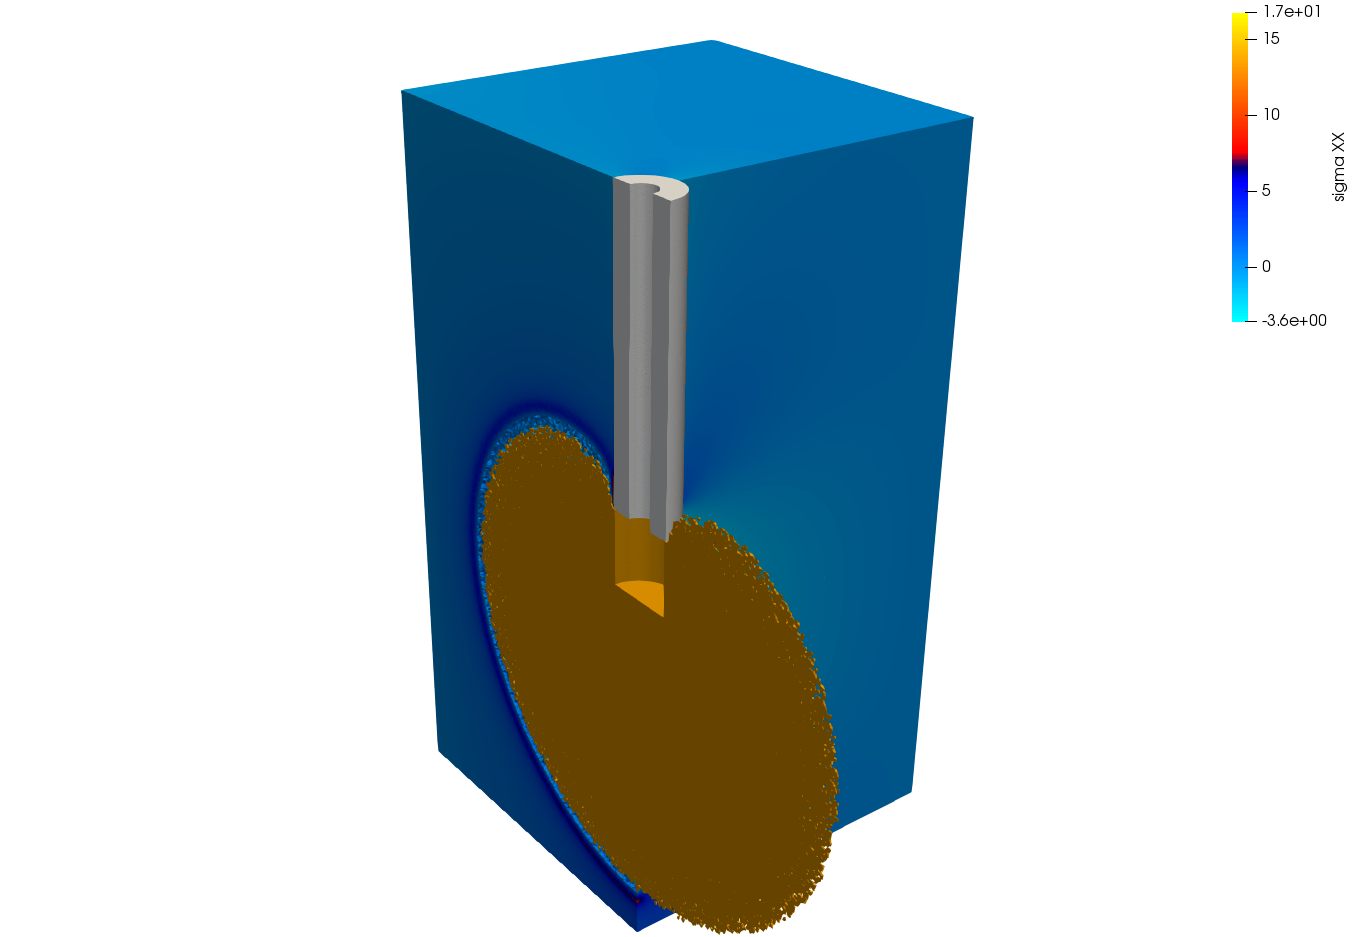
\includegraphics[width=1\textwidth]{figures/VPF_ME2_case2.png}
\caption{The simulation of fluid driven percolation for case2. Created fracture and the horizontal stress are shown.}
\label{fig:Keita_ME2_VPF_case2}
\end{figure}

\begin{figure}[!ht]
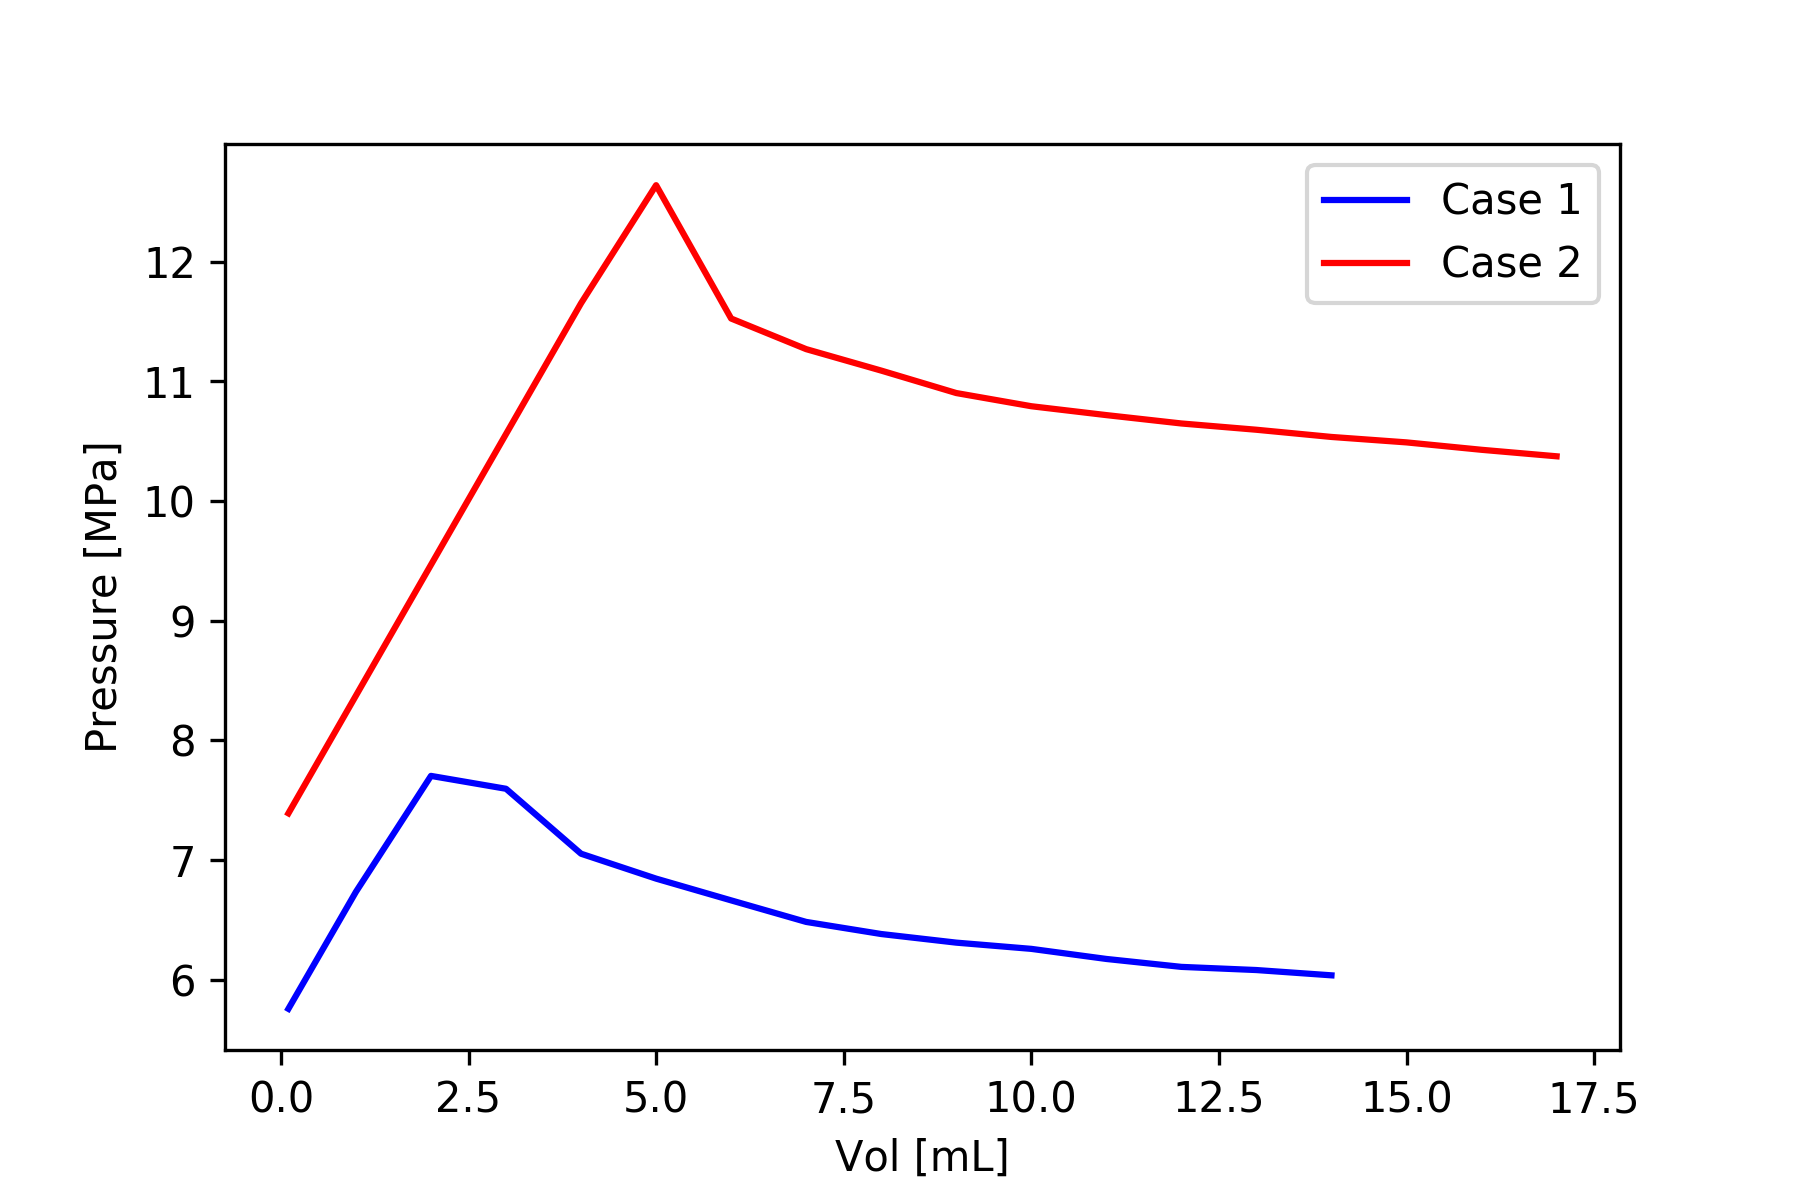
\includegraphics[width=1\textwidth]{figures/VPF_ME2_pres_vol.png}
\caption{Injection ressure responses from the cases against the injected volume.}
\label{fig:Keita_ME2_VPF_pres_vol}
\end{figure}

%------------------------------------------------------------------------------
\subsection{Results and discussion}

 The stress dependent fracking path in saltstone samples due to the defined anisotropic stress configurations is investigated. To do so,  The experimental data are taken from the literature and the validation of the numerical models is performed. 
 The VPF results of  $1^{st}$ and $2^{nd}$ stress configurations are shown in Figs~\ref{fig:Keita_ME2_VPF_case1} and~\ref{fig:Keita_ME2_VPF_case2}, respectively.
 It should be noted that in the variational phase-field method, crack nucleation or propagation is not prescribed and they will be chosen as the result of the minimization of the energy.
 The implementation in this study adopts an anisotropic energy formulation -- compression and tension split -- to be able to distinguish the compressional contribution from the tensile one.
 Thus, even though the entire system in these experiments are under compression, the evolution of the phase-field (damage) is promoted where the material experiences tension.
 
 For $1^{st}$ case, with the vertical stress being the least stress, a more or less horizontal crack propagates towards the boundary of the sample.
 As the stress concentration is induced at the bottom of the injection borehole, the crack was initiated at that point (enough tensile strain is achieved) with some angle and gradually turned to align with the horizontal plane (Fig~\ref{fig:Keita_ME2_VPF_case1}).
 The plane orthogonal to the minimum stress direction for $2^{nd}$ is the vertical plane.
 Crack propagation on that plane can be observed and its propagation is hinged by the presence of the casing tube in the borehole (Fig~\ref{fig:Keita_ME2_VPF_case2}).
 In both cases, similar pressure responses against the injected volume can be observed (Fig.~\ref{fig:Keita_ME2_VPF_pres_vol}). 
 The peak pressures observed in these cases are 12.6 and 7.7 $MPa$ and these values are proportional to the fracture toughness values input to the simulation.
 As the fracture toughness of the salt stone samples were not available in the original literature, 100 $Pa \cdot m$ was used in the simulations. 
 
 The implemented lattice model depicts the fracking paths in Fig.  \ref{fig:Amir_ME2_LEM_a_model_Fracture} and \ref{fig:Amir_ME2_LEM_b_model_Fracture}. For a $1^{st}$ and $2^{nd}$ stress configurations the fracking pressure is found to be 13.2 and 7.1 $MPa$, respectively. Both values are slightly higher than the given fracking pressure from the literature. However, the fracking pressures in both cases are higher than the minimum principle stresses. The fracking paths shown with red surfaces match the experimental results, where the $1^{st}$ stress configurations results in horizontal fracking paths and the $2^{nd}$ stress configurations results in vertical fracking paths. The discrete element method is also able to simulate the fracking path similar to the experimental results. The application of the numerical methods for quantitative comparison of the simulation results with the experimental data needs further investigation. 
